\documentclass[8pt]{beamer}
\usepackage{amsmath}
\usepackage{amssymb}
\usepackage{graphicx}
\usepackage{hyperref}
\usepackage{color}
\usepackage{float}
\usepackage{subfig}

\title{Exploring polymer models to explain the appearance of TADs}
\author{Ofir Shukron}
\institute{Ecole Normale Superieure}
\usetheme{Madrid}
\usecolortheme{dolphin}

\begin{document}

\begin{frame}{Stochastic Simulation of Topologically Associating Domains}
\titlepage
\end{frame}
\tableofcontents

\section{The experimental setting}
\begin{frame}{Chromosome Conformation Capture (3C) and its relatives}
A method to simultaneously record millions of looping events occurring within the genome. 

The 4C/5C/HiC are all derived from the 3C method and uses a 3C segment library for subsequent steps.

The general 3C steps are:
\begin{enumerate}
\item intact nuclei are extracted from millions of cells 
\item Formaldehyde induces protein-DNA and protein-protein cross-links
\item restriction enzymes digest the cross-linked DNA
\item DNA is diluted and ligated
\item cross-links are reversed
\item PCR to amplify ligation junctions
\item histogram of segment encounter is produced
\end{enumerate}
\begin{figure}{H}
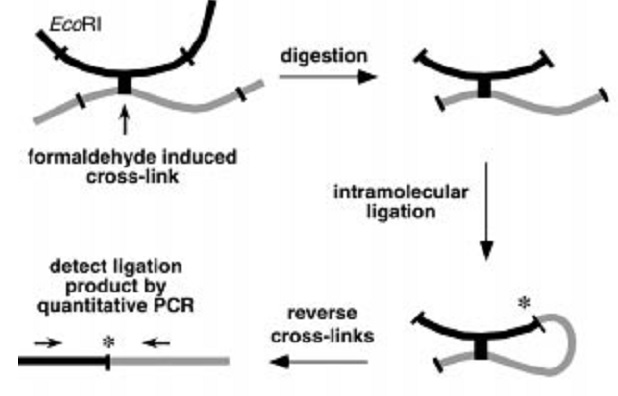
\includegraphics[scale=0.3]{3Cschematic}
\end{figure}
 
\end{frame}

\section{The data}
\begin{frame}{The data}
\begin{itemize}
\item 5C experiments were conducted by Nora et. al 2012. 
\item A subset of the data, showing X-chromosome self interactions in mouse embryonic stem cells, will be analyzed here. 
\item The focus is on regions harboring the Xist enhancer and Tisx promoter, related to X inactivation mechanism. 
\item A total length of 920,432 bp.
\item Two replicates of the experiment were made. 
\item we have the encounter matrix of different segments.
\end{itemize}
\end{frame}

\begin{frame}{Topologically Associating Domains (TADs)}
\centering
\begin{figure}\label{fig:TADsOfTheXChromosome_NoraEtAl2012}
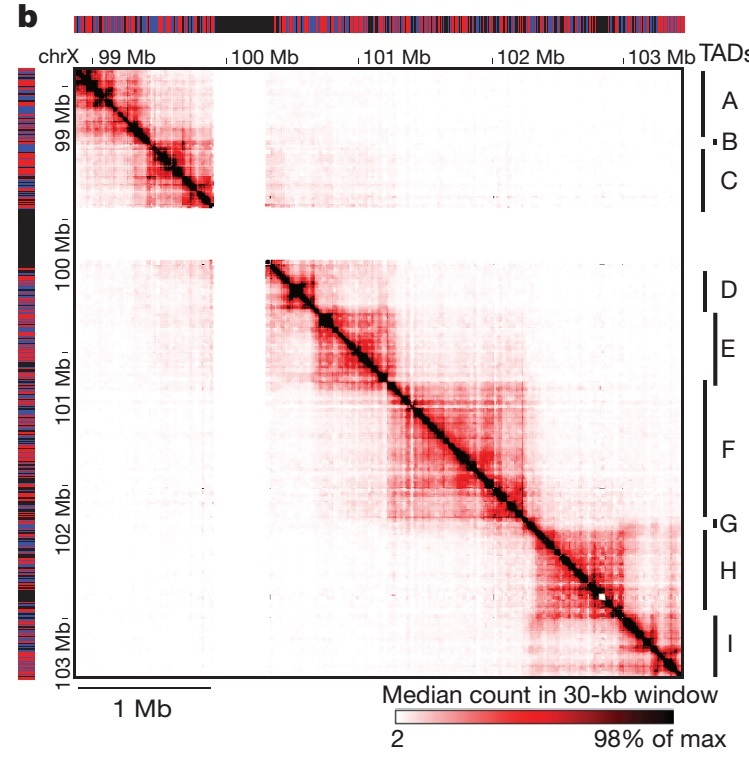
\includegraphics[scale=0.2]{TADsOfTheXChromosome_NoraEtAl2012}
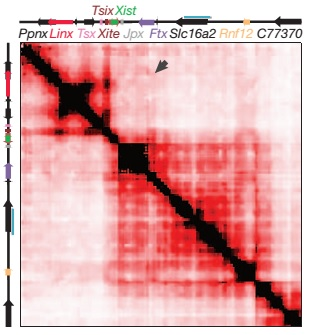
\includegraphics[scale=0.3]{TadDandENoraEtAl2012}
\caption{The 4.5 Mb region analyzed by Nora et al, and TAD D and E regions. Displayed median count in a 30kb window every 6kb}
\end{figure}
\end{frame}


\begin{frame}{From restriction segments to beads}
\begin{itemize}
\item To coarse-grain the data, Luca et. al. chose a bead-length of 3000 bp, corresponding to the mean restriction segment length of EcoRIII enzyme. 
\begin{figure}[H]
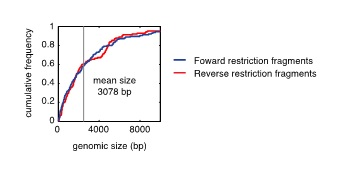
\includegraphics[scale=0.45]{restrictionSegmentLengthDistributionLucaetal}
\end{figure}
\item the genomic section was evenly partitioned by 3000 bp beads. Each segment receives a start and end index according to the beads it covers. 
\item for example, 
\begin{tabular}[H]{|l| l| l|}
\hline
bp range & start ind & end ind\\
\hline
500-3500   & 1         & 2 \\
4000-4500  & 2         & 2 \\   
5000-12001 & 2         & 4 \\       
\hline  
\end{tabular}
\end{itemize}
\end{frame}

\section{Analysis of the data}
\subsection{TAD D and E}
\begin{frame}{Analysis of the data}
\framesubtitle{TAD D and E}
\begin{itemize}
\item A total length of 920,432 bp - resulting in 307 beads
\item We calculate the 'one-sided' encounter probability vs distance (bead units) for each bead
\item the mean encounter probability difference, shows that the data is left-right symmetric
\begin{figure}[H]
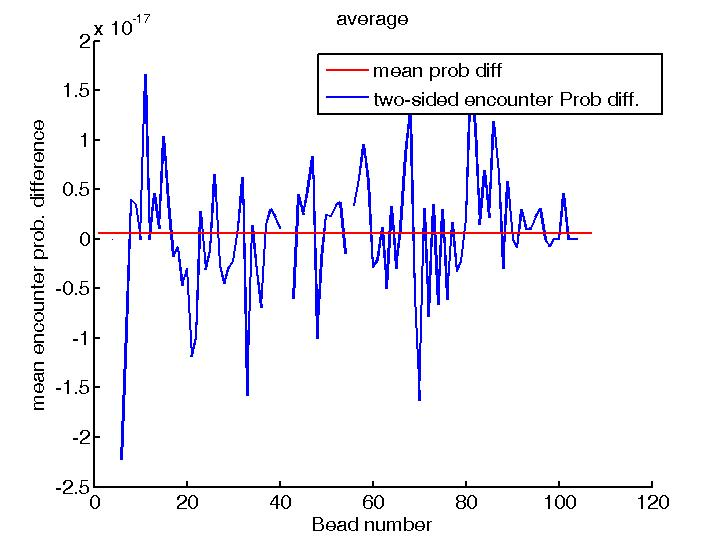
\includegraphics[scale=0.1]{symmetryOftheEncounterProbTADDAverage}
\end{figure}
\item the encounter data showed 
\end{itemize}

\begin{figure}[H]\label{TADDAndEencounterProb}
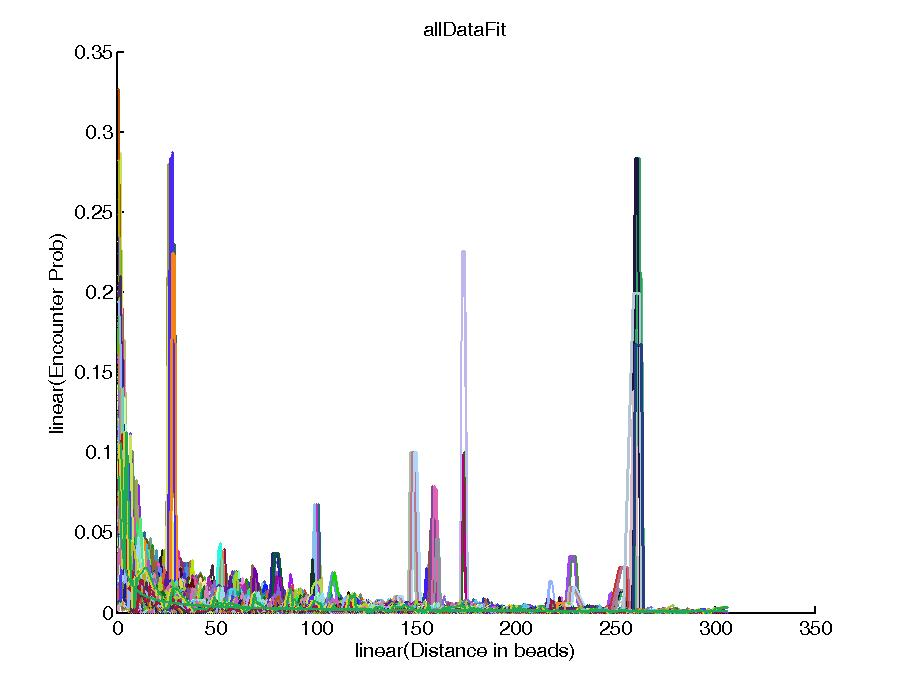
\includegraphics[scale=0.1]{encounterProbabilityTADDAndE}
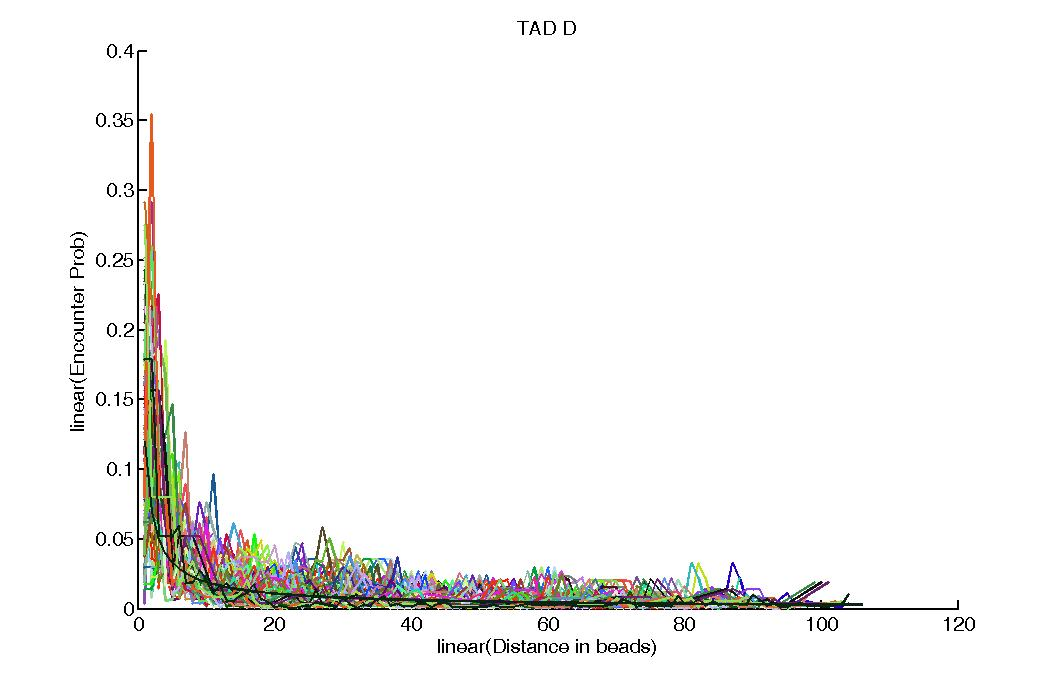
\includegraphics[scale=0.1]{encounterProbabilityTADD}
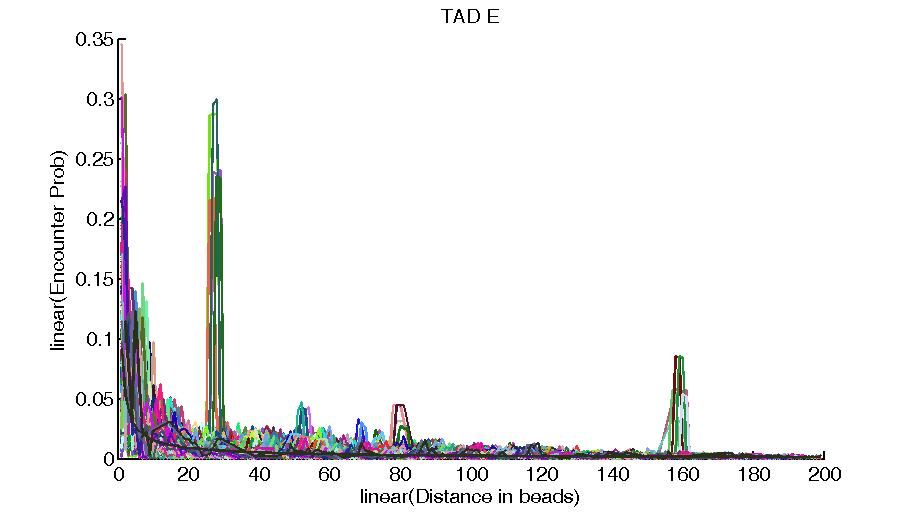
\includegraphics[scale=0.13]{encounterProbabilityTADE}
\end{figure}
\begin{itemize}
\item TAD E has several strong specific interactions.
\item TAD D has almost no specific interactions. 
\end{itemize}
\end{frame}

\subsection{Peaks of the encounter data}
\begin{frame}{Peaks of the encounter data}
\begin{itemize}
\item About half of the peaks in the encounter data result from specific interactions \textcolor{red}{between TADs}
\item The other half comes from specific internal interactions of \textcolor{green}{TAD E}.
\item To get an impression, a manual marking of the peaks shows 
\end{itemize}
\begin{table}[H]\label{nonNeighborBeadEncounterTable}
\begin{tabular}{l l l}
Bead numbers & Encountered beads & TAD\\
\hline

23-26   & 280-290 & \textcolor{red}{$D\leftrightarrow E$}\\
49-53   & 148-155 & \textcolor{red}{$D\leftrightarrow E$}\\
56-59   & 80-90   & $D\leftrightarrow D$\\
115-117 & 165-170 & \textcolor{green}{$E\leftrightarrow E$}\\
161-162 & 187 190 & \textcolor{green}{$E\leftrightarrow E$}\\
182-184 & 260-264 & \textcolor{green}{$E\leftrightarrow E$}\\
185-186 & 253-255 & \textcolor{green}{$E\leftrightarrow E$}\\
234-236 & 184-189 & \textcolor{green}{$E\leftrightarrow E$}\\
234-236 & 4-11    & \textcolor{red}{$E\leftrightarrow D$}\\
243     & 88      & \textcolor{red}{$E\leftrightarrow D$}\\
264     & 89-90   & \textcolor{red}{$E\leftrightarrow D$}\\
274-277 & 113-120 & \textcolor{green}{$E\leftrightarrow E$}
\end{tabular}
\end{table} 
\end{frame}

\section{Theoretical model}
\begin{frame}{Theoretical models}
\framesubtitle{The Rouse model}
We start with the classical and most simple model, the Rouse chain.
\begin{itemize}
\item A Rouse chain describes polymer dynamics as a stochastic motion of a collection of microscopic "beads" connected by harmonic springs
\item the 3D  motion of bead $n$ in the chain of $N$ beads 
\begin{equation*}
\frac{dR_n}{dt} = -\frac{3D}{b^2}(2R_n(t)-R_{n+1}(t)-R_{n-1}(t))+f_n(t)
\end{equation*}
\item $R_n$- the position of bead $n$\\
$b$- the standard deviation of the distance between adjacent beads\\
$D$- the diffusion constant\\
$f_n$- white Gaussian noise
\item From the theory, $Pr(\|R_n-R_m\|<\epsilon)\sim  |n-m|^{-1.5}$
\end{itemize}
\end{frame}

\section{Simulations}
\subsection{Simulations with a simple rouse chain}
\begin{frame}{Simulation with simple rouse chain}
\begin{itemize}
\item we first check whether a simple model can produce the TADs. 
\item we examine the results of simulating  chain of 64 beads
\end{itemize}

\end{frame}

\subsection{Loops corresponding to the peaks of the encounter data}
\begin{frame}{Loops corresponding to the peaks of the encounter data}

\end{frame}

\subsection{Dynamic loops model}
\begin{frame}{Dynamic Loop Model}
\begin{itemize}
\item some beads in the same TAD have affinity toward one another
\item affine beads located within a distance less than $\epsilon$ (the encounter distance) are connected
\item the rate of disconnection between beads is $k_{off}$
\end{itemize}
\end{frame}

\subsection{Dynamic loops model with beads' affinity}
\begin{frame}{Dynamic loops model with beads affinity}
\end{frame}

\subsection{Enlarging the encounter distance}
\begin{frame}{Enlarging the encounter distance}
\end{frame}

\subsection{3C experiment with stiff connectors}
\begin{frame}{3C experiment with stiff connectors}
Next, we simulate 64 bead chains with stiff connectors.\\
Stiff connectors are Rouse spring that stay fixed.\\
\end{frame}

\section{Future Perspectives}
\begin{frame}{Future perspective}
\begin{itemize}
\item A model with variable encounter distance
\item 
\end{itemize}
\end{frame}

\end{document}